\section{Keyword-Driven Testing}

Keyword-driven testing is a logical extension to data-driven testing~\cite{Fewster99}.
Besides test data, it also makes use of keywords in order to instruct how the
data is read from the external data source and to be interpreted by the test
scripts. It takes the concept of data-driven testing even further~\cite{Lau07}
by adding keywords driving the test executing into the test data with the desire
to be able to specify automated test cases without having to specify all the
excessive detail. The test data file is expanded and it becomes a description of
the test case using a set of keywords to indicate the tasks to be performed.
Obviously, the driver script has to be able to interpret the keywords in order
to execute the desired test case.

Back to the previous scenario on data-driven testing where the operation
10 * 5 - 5 = 45 would require major changes to both test data and driver
scripts. The keyword-driven testing is the perfect technique to perform that
kind of scenarios. They could be extended with no further development since the
keywords are already implemented by the driver script. This way, the driver
script is no longer tied to a particular feature of the software under test,
nor indeed to a particular application or system~\cite{Fewster99}.

This technique takes a descriptive approach to test case implementation since
the test file describes the test case, by stating what the test case does and
not how it does it. To implement an automated test case we have only to provide
a description of the test case more or less as we would do for a knowledgeable
human tester. By using this approach we can build knowledge of the system under
test into our test automation environment. People with business knowledge can
concentrate on the test files while people with technical skills can concentrate
on the driver scripts since it is possible to develop the test cases separately
from the test scripts due to the abstraction created by the test files.

\subsection{Test data}

\begin{table}[!ht]
\centering
\begin{tabular}{lll}
\textbf{Test Case} & \textbf{Keyword} & \textbf{Value} \\
\textbf{Addition 01} & & \\
& Operand & 5 \\
& Operator & + \\
& Operand & 5 \\
& Result & 10 \\
\textbf{Addition 02}  & & \\
& Operand & 5 \\
& Operator & + \\
& Operand & 10 \\
& Operator & - \\
& Operand & 1 \\
& Result & 14 \\
\end{tabular}
\caption{Keyword-driven test data with mathematical operations.}
\label{table:tab2}
\end{table}

\noindent There is no real difference between handling keyword-driven and data-driven test
data~\cite{Fewster99}~\cite{Lau07}, but we need to make a big decision when designing a keyword-driven framework:
the abstraction level of the keywords to be used~\cite{Lau07}. When testing higher level
functionality like business logic, low level keywords tend to make test cases
very long, defined on Table \ref{table:tab2}, while higher level keywords, defined
on Table \ref{table:tab3} are much more usable. These higher level keywords shouldn't
be implemented directly into the framework. Instead, they should be implemented
using the same technique used for designing test cases. The main benefit in
making it possible to create new keywords using the test design system is that
they can be created and maintained easily without any programming skills. The
drawback~\cite{Lau07} from this approach is that the driver script will get more
complex since it has to handle two kinds of keywords.

\begin{table}[!ht]
\centering
\begin{tabular}{lll}
\textbf{Test Case} & \textbf{Keyword} & \textbf{Value} \\
\textbf{Addition 01} & & \\
& Input & 5 \\
& Add & 5 \\
& Result & 10 \\
\textbf{Addition 02} & & \\
& Input & 5 \\
& Add & 10 \\
& Subtract & 1 \\
& Result & 14 \\
\end{tabular}
\caption{Keyword-driven test data with higher level keywords.}
\label{table:tab3}
\end{table}

\subsection{Processing test data}

The driver script should be very similar to
the one presented in Listing \ref{lst:lis1} and must be able to interpret the defined
keywords and execute the matching action using the assigned values. Generally the number of scripts required for this approach is a function of the
size of the software under test rather than the number of tests~\cite{Fewster99}.

\begin{lstlisting}[caption={Example of keyword-driven driver script.},
    label={lst:lis2},language=JavaScript]
const TestData = require('./testData');
const Calculator = require('./calculator');

TestData.testCases().forEach(function(testCase) {
  testCase.keywords().forEach(function(keyword, value) {
    execute(keyword, value);
  });
});
\end{lstlisting}

\begin{figure}[!ht]
\centering
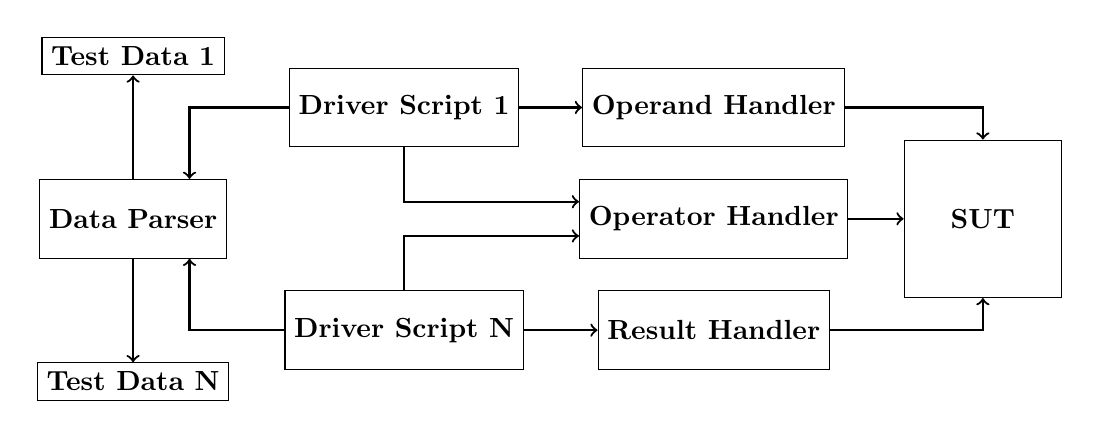
\begin{tikzpicture}
\matrix [column sep=7mm, row sep=-1mm] {
  \node (data1) [draw, shape=rectangle] {\textbf{Test Data 1}}; & & & \\
  & \node (script1) [draw, shape=rectangle,minimum width=2cm,
  minimum height=1cm] {\textbf{Driver Script 1}}; & 
  \node (tscript1) [draw, shape=rectangle,minimum width=2cm,
  minimum height=1cm] {\textbf{Operand Handler}}; \\
  \node (parser) [draw, shape=rectangle,
  minimum width=2cm, minimum height=1cm] {\textbf{Data Parser}}; & &
  \node (tscript2) [draw, shape=rectangle,minimum width=2cm,
  minimum height=1cm, align=left] {\textbf{Operator Handler}}; &
  \node (sut) [draw, shape=rectangle, minimum width=2cm,
  minimum height=2cm] {\textbf{SUT}}; \\
  & \node (scriptn) [draw, shape=rectangle,minimum width=2cm,
  minimum height=1cm] {\textbf{Driver Script N}}; & 
  \node (tscriptn) [draw, shape=rectangle,minimum width=2cm,
  minimum height=1cm] {\textbf{Result Handler}}; \\
  \node (datan) [draw, shape=rectangle] {\textbf{Test Data N}}; & & \\
};
\draw[->, thick] (parser) -- (data1);
\draw[->, thick] (parser) -- (datan);
\draw[->, thick] (script1) -| ([xshift=2cm,yshift=5mm]parser);
\draw[->, thick] (scriptn) -| ([xshift=2cm,yshift=-5mm]parser);
\draw[->, thick] (script1) -- (tscript1);
\draw[->, thick] (script1) |- ([yshift=5mm]tscript2);
\draw[->, thick] (scriptn) |- ([yshift=-5mm]tscript2);
\draw[->, thick] (scriptn) -- (tscriptn);
\draw[->, thick] (tscript1) -| (sut);
\draw[->, thick] (tscript2) -- (sut);
\draw[->, thick] (tscriptn) -| (sut);
\end{tikzpicture}
\caption{Keyword-driven system design approach.} \label{fig:f2}
\end{figure}

In this keyword-driven approach there are a few elements that are crucial and must be implemented:
\begin{itemize}
\item \textbf{Data Parser}: Share the same responsibility as the data-driven parser defined on Figure \ref{fig:f1}, but has to handle multiple instructions per test case (Input, Add, Result).
\item \textbf{Driver Script}: Share the same responsibility as the data-driven driver defined on Figure \ref{fig:f1}, but instead of dealing directly with the test libraries, it needs to use specific handlers to translate the keywords and the data values that are read by the data parser in order to execute the tests.
\item \textbf{Handlers}: Each action keyword corresponds to a single fragment of a test script (Operator, Operand, and Result handler), allowing the test execution tool to translate a sequence of keywords and data values into executable tests.
\end{itemize}

\subsection{Advantages of keyword-driven testing}

Keyword-driven testing has all the same benefits as data-driven testing since it
shares the same principle of making easier to create new kinds of tests, even
for non-programmers. But despite their resemblances, keyword-driven testing is
a big step forward from pure data-driven testing where all tests are similar and
creating new tests always require new code in the framework. Once the basic
driver scripts are in  place, it is possible to implement thousands of test
cases with only a few hundred test scripts. This approach not only speeds up the
implementation of automated tests, but also makes it possible to use testers
without programming skills to implement them. The beauty of this approach is
that it can be implemented in a tool independent way so that we can re-implement
the driver scripts in another testing tool or programming language without
loosing the investment in the test cases. All of the information about what to
test is now contained in the data table, so the separation of test information
from implementation is the greatest advantage in this technique.

\subsection{Disadvantages of keyword-driven testing}

The main problem with the keyword-driven approach is that test cases tend to get
longer and more complex than when using the data-driven approach. If we look at
the example from Table \ref{table:tab1}, the test case Addition 01 has only
one line and it's very restrictive in terms of inputs. On the other hand, the
same test case on Table \ref{table:tab2} has four lines, is more complex to
implement, but has lot more flexibility.